% Compile with XeLaTeX or Tectonic. Keep portrait.png in the same folder.
\documentclass[10pt,a4paper]{article}
\usepackage[a4paper,left=12mm,right=12mm,top=10mm,bottom=13mm]{geometry}
\usepackage{fontspec}
\setmainfont{lmroman10-regular.otf}[BoldFont=lmroman10-bold.otf,ItalicFont=lmroman10-italic.otf,BoldItalicFont=lmroman10-bolditalic.otf]
\usepackage{graphicx}
\usepackage{enumitem}
\usepackage{titlesec}
\usepackage{hyperref}
\hypersetup{hidelinks,pdftitle={CV - Ưng Nhựt Khang - Web Developer},pdfauthor={Ưng Nhựt Khang}}
\pagestyle{empty}
\setlength{\parindent}{0pt}
\setlength{\parskip}{0pt}
\setlist[itemize]{leftmargin=12pt,itemsep=1pt,topsep=2pt,parsep=0pt}
\titleformat{\section}{\fontsize{12.5}{15}\selectfont\bfseries}{}{0pt}{}[\vspace{1pt}\titlerule]
\titlespacing*{\section}{0pt}{7pt}{4pt}
\newcommand{\project}[2]{\textbf{#1}\hfill #2\par}
\newcommand{\projectmeta}[2]{{\fontsize{9}{11}\selectfont\itshape #1\hfill #2}\par}
\begin{document}
\fontsize{10}{12}\selectfont

\begin{minipage}[c]{28mm}
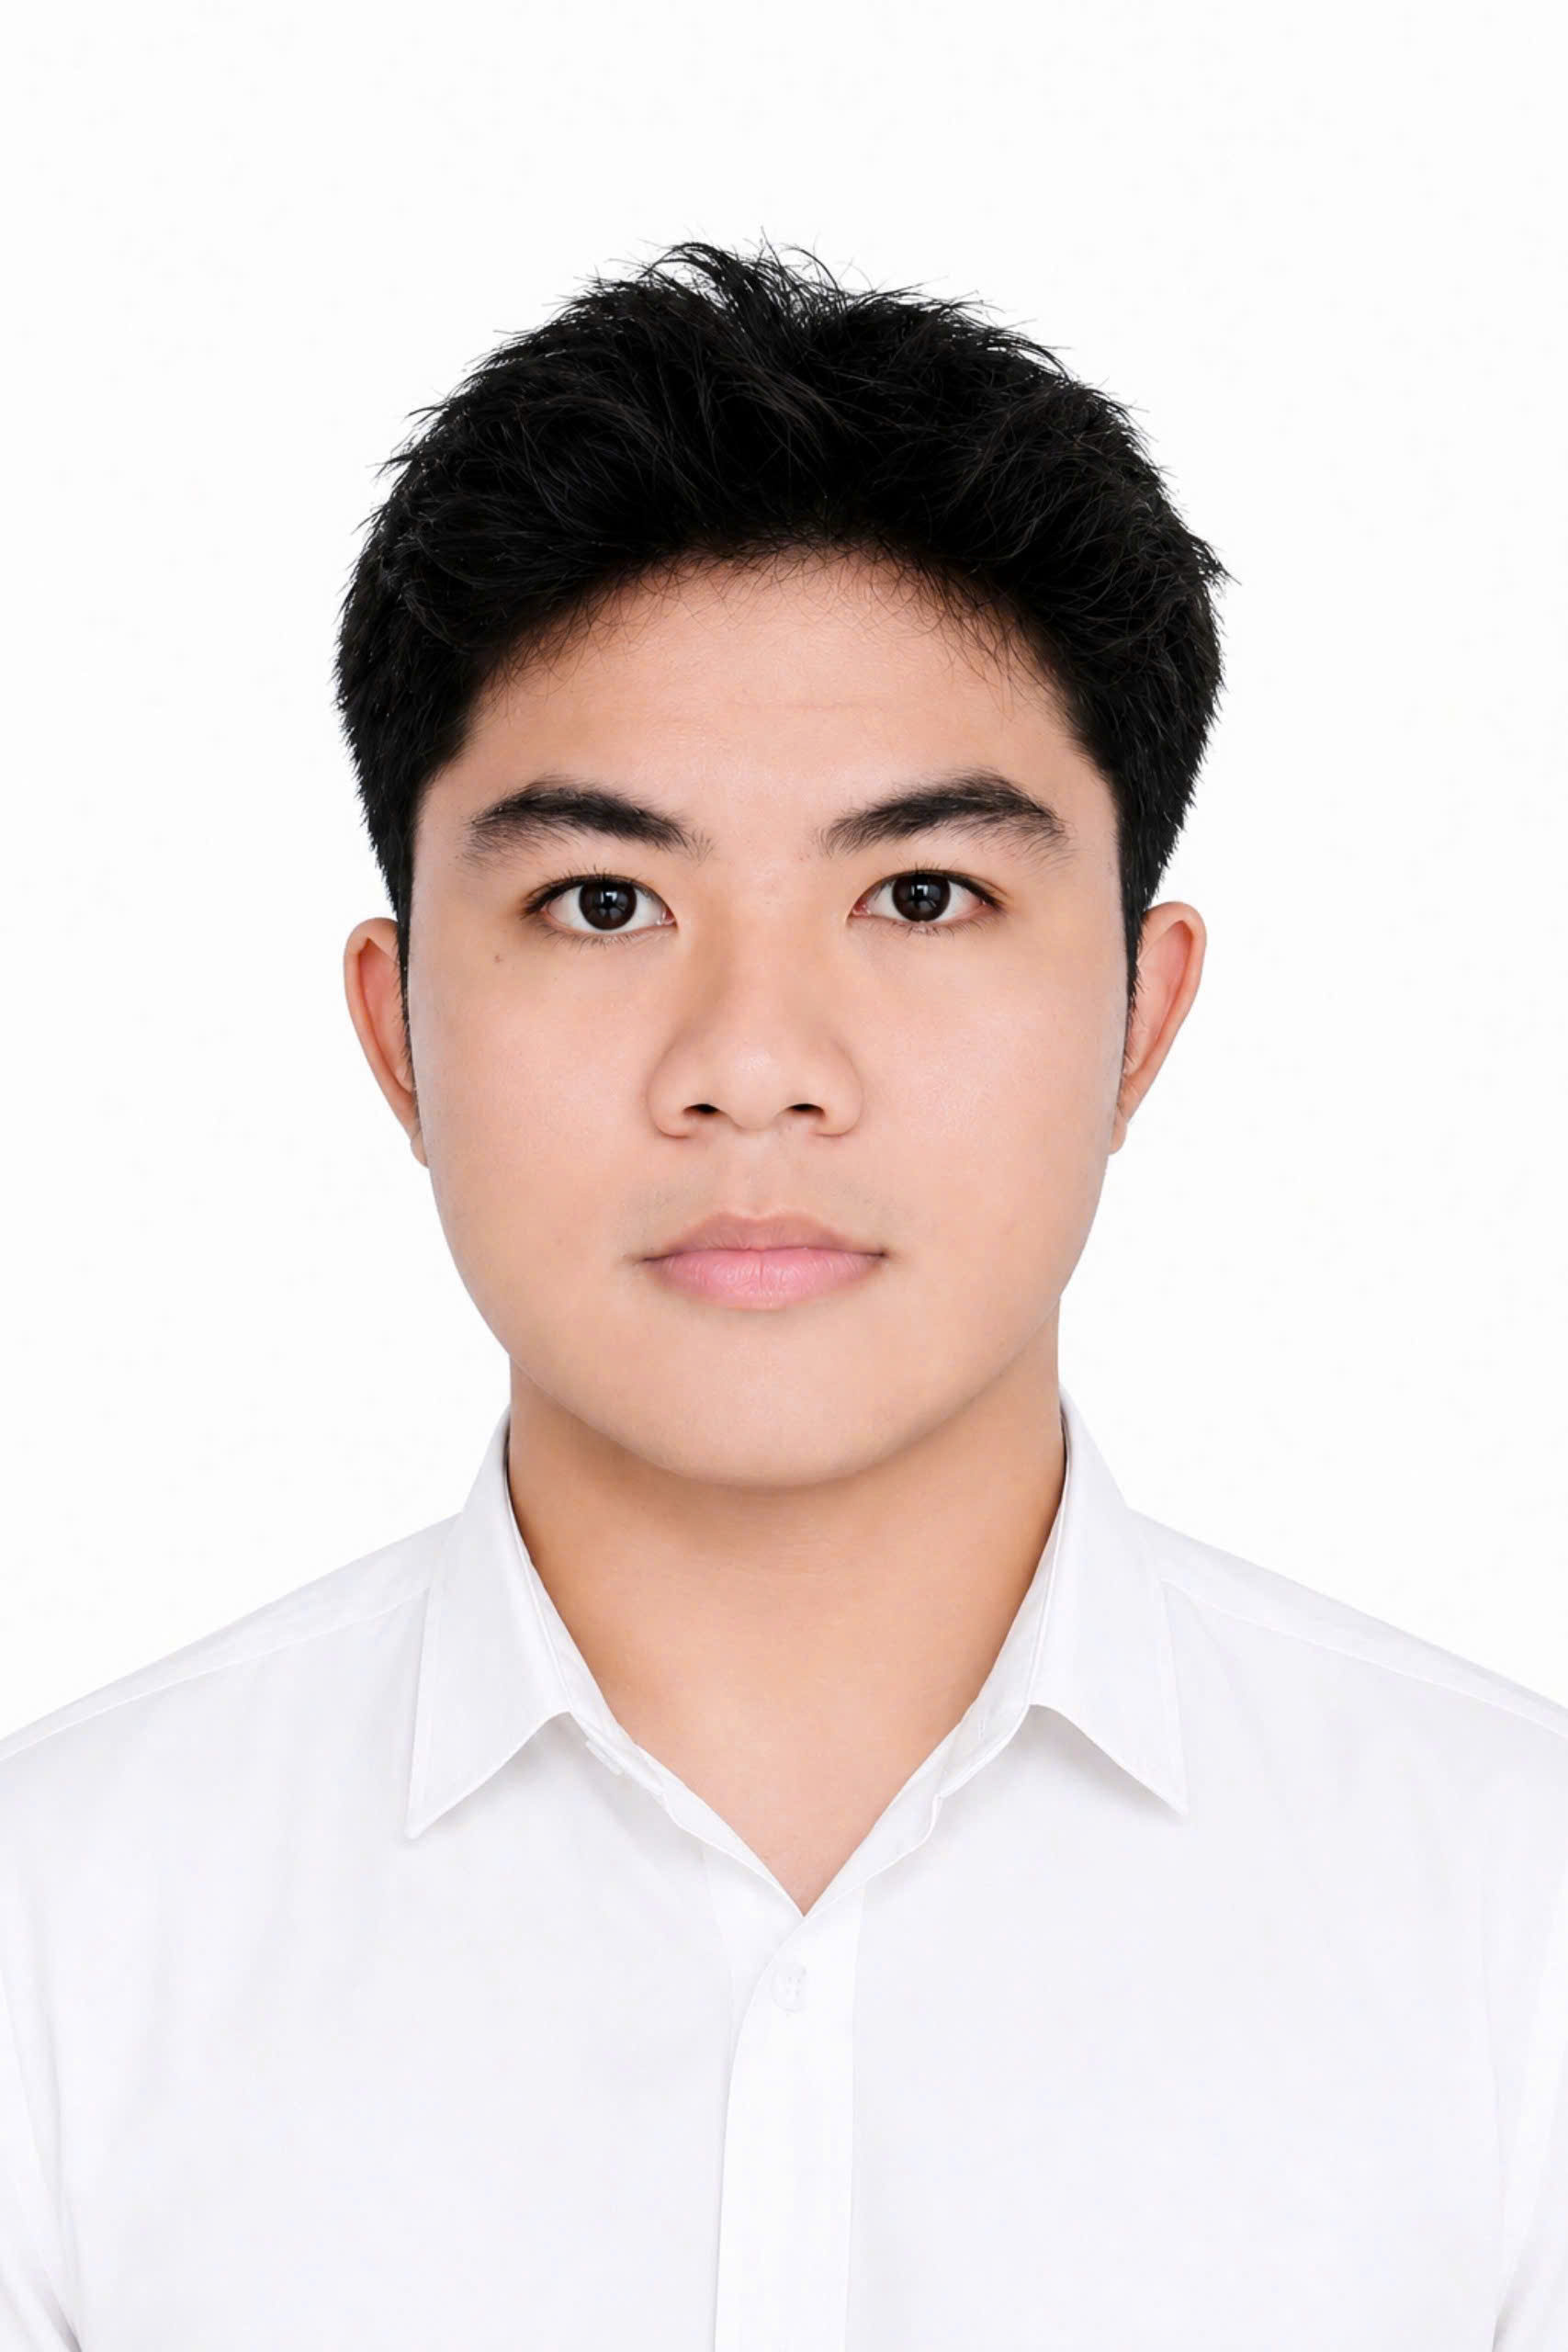
\includegraphics[width=28mm]{../site/public/profile.jpg}
\end{minipage}\hspace{4mm}%
\begin{minipage}[c]{153mm}
{\fontsize{19}{23}\selectfont\bfseries ƯNG NHỰT KHANG}\par
\vspace{3pt}
{\fontsize{10.5}{13}\selectfont\bfseries Web Developer}\par
\vspace{3pt}
Sinh viên Công nghệ thông tin, chuyên ngành Kỹ thuật phần mềm\par
\vspace{5pt}
\textbf{Email:} \href{mailto:contact@ungnhutkhang.id.vn}{contact@ungnhutkhang.id.vn}\hspace{5mm}\textbf{Điện thoại:} 0393 331 566\par
\vspace{2pt}
\textbf{Địa chỉ:} Phường Cát Lái, TP. Hồ Chí Minh\par
\vspace{2pt}
\textbf{GitHub:} \href{https://github.com/mm4you}{github.com/mm4you}\par
\vspace{2pt}
\textbf{Website:} \href{https://www.ungnhutkhang.id.vn/}{ungnhutkhang.id.vn}
\end{minipage}
\vspace{5pt}
\hrule height 0.4pt
\vspace{5pt}

\section{Mục tiêu nghề nghiệp}
Sinh viên Kỹ thuật phần mềm tại UMT, tìm kiếm cơ hội thực tập phát triển Web. Thực hành React, Next.js, TypeScript, cơ sở dữ liệu và tích hợp API qua các dự án cá nhân và dự án nhóm. Chủ động tự học, sử dụng AI hỗ trợ lập trình và mong muốn đóng góp trong môi trường làm việc thực tế.

\section{Học vấn}
\textbf{Trường Đại học Quản lý và Công nghệ TP. Hồ Chí Minh (UMT)}\hfill 2024 - hiện tại\par
\textit{Ngành Công nghệ thông tin, chuyên ngành Kỹ thuật phần mềm (Software Engineering, SE)}
\begin{itemize}
\item GPA hiện tại: \textbf{3.31}. Dự kiến tốt nghiệp năm \textbf{2028}.
\end{itemize}

\section{Dự án}
\project{IELTS Vocabulary}{\href{https://ielts.vocab.umters.club/}{Trải nghiệm} / \href{https://github.com/mm4you/ielts}{GitHub}}
\projectmeta{Ứng dụng học từ vựng IELTS}{Next.js, TypeScript, Tailwind CSS, Prisma, PostgreSQL}
\begin{itemize}
\item Ôn tập theo thuật toán SM-2, trò chơi luyện tập và phát âm; hỗ trợ đăng nhập, lưu dữ liệu và theo dõi tiến độ.
\end{itemize}
\vspace{2pt}
\project{InnovateX Smart Port}{2025 / \href{https://github.com/mm4you/hackathon}{GitHub}}
\projectmeta{Hackathon Digiport Logistics 2025}{Next.js, TypeScript, Prisma, PostgreSQL}
\begin{itemize}
\item Đặt lịch vào cảng, quản lý lịch hẹn, bảng điều khiển vận hành và điểm thưởng xanh. \textbf{Top 20 (Bán kết)} Hackathon Digiport Logistics 2025.
\end{itemize}
\vspace{2pt}
\project{Vô Tri}{\href{https://votrihub.vercel.app/}{Trải nghiệm} / \href{https://github.com/mm4you/votri}{GitHub}}
\projectmeta{Cổng trò chơi trên trình duyệt}{JavaScript, Three.js, Web Audio API, HTML, CSS}
\begin{itemize}
\item Splash Swim và Wobbly Bird với cảnh 3D, xử lý vật lý và âm thanh; hỗ trợ Việt/Anh, lưu thiết lập và thành tích trên trình duyệt.
\end{itemize}
\vspace{2pt}
\project{Thi Thố - Đường lên đỉnh tri thức}{\href{https://thitho.vercel.app/}{Trải nghiệm} / \href{https://github.com/mm4you/thitho}{GitHub}}
\projectmeta{Hệ thống gameshow thời gian thực}{Next.js, TypeScript, Supabase Realtime, Tailwind CSS}
\begin{itemize}
\item Thi đấu kiến thức cho bốn người chơi, bảng điều khiển MC/giám khảo và màn hình sân khấu; đồng bộ câu trả lời, đồng hồ, điểm số; hỗ trợ bấm chuông và chấm điểm.
\end{itemize}
\vspace{2pt}
\project{Drive Music}{\href{https://github.com/mm4you/drive-music}{GitHub}}
\projectmeta{Trình nghe nhạc trên web}{React, Next.js, Media Session API, PWA}
\begin{itemize}
\item Phát nhạc FLAC, quản lý danh sách phát và điều khiển màn hình khóa; giao diện responsive, hỗ trợ cài đặt dạng PWA.
\end{itemize}
\vspace{2pt}
\project{CSVC UMT (Quản lý cơ sở vật chất)}{\textit{Đang phát triển}}
\begin{itemize}
\item Dự án nhóm phát triển ứng dụng web quản lý cơ sở vật chất tại UMT. Vai trò: Thành viên phát triển.
\end{itemize}

\section{Kỹ năng chuyên môn}
\begin{tabular}{@{}p{37mm}@{\hspace{3mm}}p{146mm}@{}}
\textbf{Frontend:} & JavaScript, TypeScript, React, Next.js, Tailwind CSS, Responsive UI.\\[3pt]
\textbf{Backend:} & Next.js API Routes, RESTful API, Prisma ORM, xác thực cơ bản (Auth).\\[3pt]
\textbf{Cơ sở dữ liệu:} & PostgreSQL, MySQL, Supabase.\\[3pt]
\textbf{Công cụ:} & Git, GitHub, Vercel.\\[3pt]
\textbf{AI hỗ trợ lập trình:} & Sử dụng và thích nghi với công cụ AI để tra cứu, hỗ trợ viết mã và gỡ lỗi.\\[3pt]
\textbf{Tiếng Anh:} & B1-B2 (tự đánh giá, chưa có chứng chỉ).
\end{tabular}

\section{Sở thích}
Gặp gỡ bạn bè, trò chuyện, cà phê, nghe nhạc và xem phim.
\end{document}
